\documentclass[10pt,a4paper]{article}
\usepackage[latin1]{inputenc}
\usepackage{amsmath}
\usepackage{amsfonts}
\usepackage{amssymb}
\usepackage{graphicx}
\usepackage[]{natbib}
\usepackage{hyperref}
\usepackage{bm}
\begin{document}
\title{Learning how to move by natural language instructions}	
\author{}
\date{}
\maketitle

\section{Introduction}




\section{Related Work}

The decision making of a rational agent relies on the utility optimization of a given task.
In path-planning for a robot, the common way is finding the minimum-cost path in the cost map defined by the environment.
Thus, how the cost function is defined determines how the robot walks.

\cite{5509772} converts a crowd flow to a cost function for the robot can have human-like navigating in crowds.
\cite{Ratliff:2006:MMP:1143844.1143936} applies this to ``imitation learning'', which learns the mappings from features to cost functions for decision making.

\cite{AAAI159766}

\section{A Structured Language for Cost Function}

We first define a structure language that defines a cost function from a given world.
Let the world model be a set of objects $ \bm{O} = \{ o_1 , \cdots , o_n \} $.
The cost function defined by the objects in the world model is $ F( \bm{O} ) = F( o_1 , \cdots , o_n ) $.
For an object in the world model $ o_i \in \bm{O} $, let there be a positive-definite kernel function $ K( o_i ) $.
We can use linearly weighted kernels to approximate the cost function,
\begin{equation}
\label{eq:kernel_approx}
F( o_1 , \cdots , o_n ) = \sum_{i=1}^{n} w_i K( o_i ).
\end{equation}

\begin{figure}
\centering
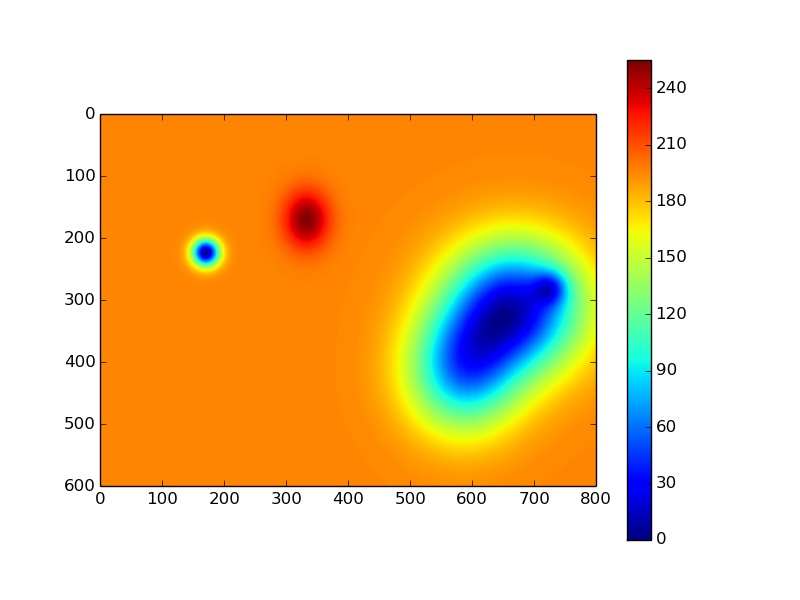
\includegraphics[width=0.6\linewidth]{fig/costmap}
\caption{A cost function of a 2D world model.}
\label{fig:costmap}
\end{figure}


\section{CDCG Model for Language Phrases}

We are looking for the cost map that best performs the activities described by an instruction $ \Lambda $ in the context of the world model $ \Upsilon $,
\begin{equation}
\label{eq:best_match:a}
\arg \max_{ F \in \bm{F} } p( F \mid \Lambda , \Upsilon ).
\end{equation}

Let the groundings be the kernels defined by the objects
$ \gamma_i = K( o_i ) $.
By applying Equation~\eqref{eq:kernel_approx} to Equation \eqref{eq:best_match:a}, we can have
\begin{equation}
\label{eq:best_match:b}
\begin{aligned}
& \arg \max_{ w_1 , \cdots , w_n } p( F \mid \Lambda, \Upsilon ) \\
= & \arg \max_{ w_1 , \cdots , w_n } p( F( w_1 , \cdots , w_n , \gamma_1 , \cdots, \gamma_n ) \mid \Lambda, \Upsilon ) \\
= & \arg \max_{ w_1 , \cdots , w_n } p'( w_1 , \cdots , w_n \mid \gamma_1 , \cdots, \gamma_n, \Lambda, \Upsilon ).
\end{aligned}
\end{equation}

By assuming that all phrases are conditionally independent and all groundings are composed of conditionally independent elements, we can have Equation~\eqref{eq:best_match:b} as
\begin{equation}
\label{eq:best_match:c}
\begin{aligned}
& \arg \max_{ w_1 , \cdots , w_n } p( F \mid \Lambda, \Upsilon ) \\
= & \arg \max_{ w_i } \prod p'( w_i \mid \gamma_i , \lambda_i, \Gamma_{c_i} , \Upsilon ).
\end{aligned}
\end{equation}

This forms a equation form close to Equation (11) in \cite{howard2014natural},
\begin{equation}
\arg \max_{ \phi_{ij} \in \Phi } \prod p( \phi_{ij} \mid \gamma_{ij} , \lambda_i , \Gamma_{c_{ij}} , \Upsilon ).
\end{equation}
Here a weight $ w_i $ corresponds to a correspondence variable $ \phi_{ij} $.
However, it is a real value instead of a boolean value.

Similarly, log-linear models are chosen to approximate the probability of a weight given the groundings and language.
We can write it as
\begin{equation}
\arg \max_{ w_i } \prod \psi ( w_i , \gamma_i , \lambda_i, \Gamma_{c_i} , \Upsilon )
\end{equation}
with
\begin{equation}
\psi ( w_i , \gamma_i , \lambda_i, \Gamma_{c_i} , \Upsilon ) = 
\frac{ e^{ \sum_{l} \mu_l f_l ( w_i, \gamma_i , \lambda_i , \Gamma_{c_i} , \Upsilon ) } }{ \int_{ w } e^{ \sum_{l} \mu_l f_l ( w, \gamma_i , \lambda_i , \Gamma_{c_i} , \Upsilon ) } } .
\end{equation}

\section{Experiments}

The experiments include
\begin{itemize}
	\item generating samples of cost functions by different weights, 
	\item verbally labeling paths from generated cost functions,
	\item and training a model with labeled samples.
\end{itemize}

\subsection{Generate Training Samples}



\subsection{Training the Model}



\bibliographystyle{apalike} 	
\bibliography{reference}
	
\end{document}